\graphicspath{{figures/analysis/}}
\chapter{Analysis}\label{ch:analysis}
To be able to both properly detect and track fish an evaluation of the state of the art solutions is necessary. This is done in regards to the already existing solution made by Loligo Systems called LoliTrack and other implementations of fish tracking in both two and three dimensions.

The chapter also presents setup and utility considerations.

\section{Fish Detection}
As stated in \autoref{sec:loligo_res} Loligo Systems extracts BLOBs from a binary image to detect the fish in an aquarium. Using the binary image with noise reduction resembles a background subtraction, as the detector has a clear distinction between objects and empty space.

Background subtraction is a common detection technique for vision applications due to the separation between wanted objects and the rest of the scene in an image. A tracker which uses this is idTracker.

Another implementation of fish tracking is to separate each fish by determining the direction in which each fish is moving by determining where the head and tail of the fish is by splitting the body of the fish into rectangles.

\subsection{idTracker}
The tracker is able to track up to 20 objects in a scene from a video sequence by annotating specific fingerprints to each object and ID'ing it that way.

Firstly each image from the video feed is normalised to its mean intensity, in which BLOBs with a mean pixel intensity outside of the set threshold are extracted. An optional background subtraction is possible using an average background image computed from the entire video.

The identification is done by comparing each BLOB extracted with reference images and compute the probability of a specific BLOB to belong to the correct ID.

\subsection{Rectangle Body Modelling}
According to [the author]\todo{insert sources when mendely is synced} the fish body is split into 8 rectangles with the same length but decreasing width to match the curvature of the fish body going from head to tail.

The implementation firstly makes a background subtraction with a background image made in the same way as from idTracker. And then converted to a binary image by using a threshold. From there the boundary of each fish is extracted.

The curvature of the fish body is computed along with detection of the nose point of the fish. by locating the two local maximums on the fish; one on the nose of the fish, which is the lower one, and one on the tail.

Head orientation is found using two points on the head curvature. The orientation is then defined as a direction perpendicular to the line between the two points. With the nose point and head orientation it is possible to place the first rectangle.

Pose estimation of the fish is done based on rectangle chain fitting. Each rectangle is fixed to a joint on the previous rectangle. The following rectangle is then rotated around the joint in a fixed amount of random angles between $0$ and $2\pi$. The rectangles are of fixed sizes and the rectangle which covers the fish the best is chosen. An example of the rectangles covering the fish is shown in \autoref{fig:rect-fish}.

\begin{figure}[h]
  \centering
  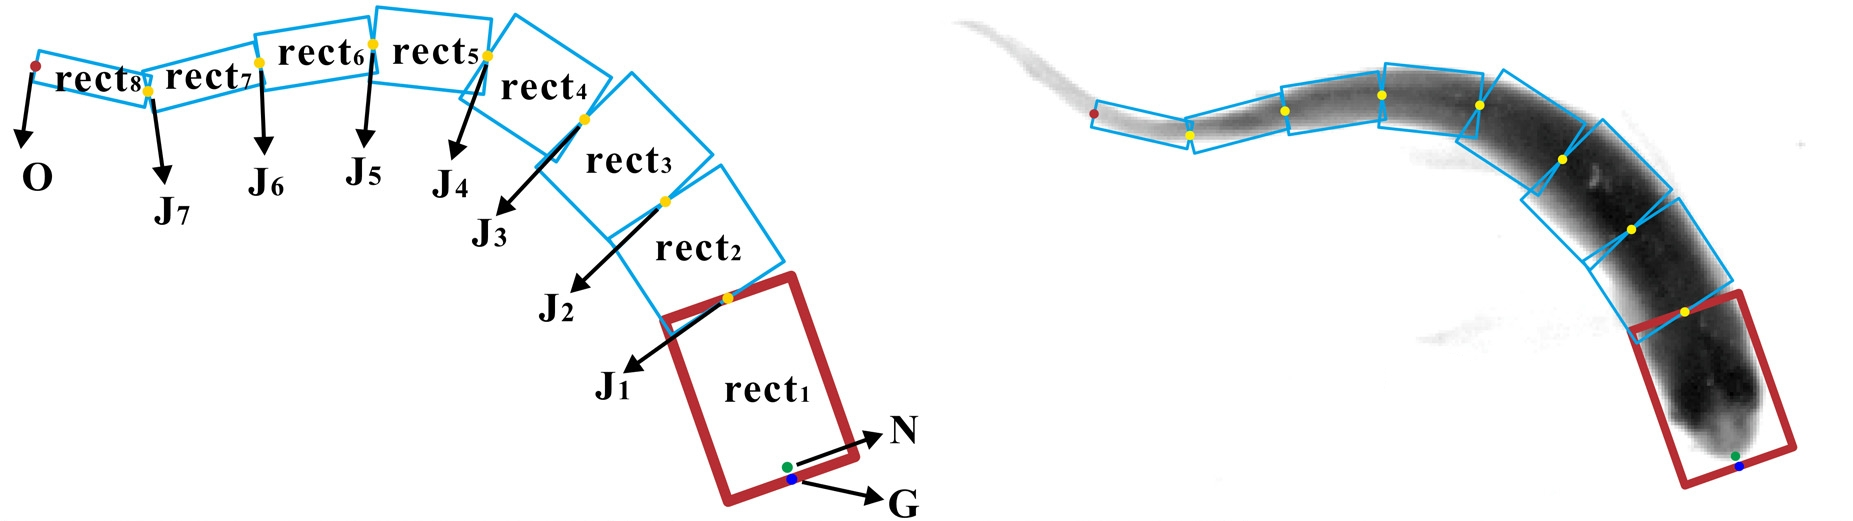
\includegraphics[width=\textwidth]{rect-fish}
  \caption{Example of rectangles covering the fish to define shape}
  \label{fig:rect-fish}
\end{figure}

\section{Fish Tracking}
